\chapter{State of the Art}
\label{chap:state_of_the_art}

\section{Cellular Structures}
\label{chap:cellular_structures}
Cellular structures are a relatively new kind of structure with promising properties that can be utilized in engineering, as they combine high stiffness with low mass. They are common in nature, such as in honeycombs, bone and wood. While they have been manufactured in the past using conventional approaches, such as using complex molds for casting \cite{Tao_Leu_2016}, their use in recent times has been accelerated due to the rise of additive manufacturing \cite{Jandyal_Chaturvedi_Wazir_Raina_Ul_Haq_2022}. Cellular structures can be broken into two categories. These are stochastic structures (foams) that have random non-repeating structures, and lattice structures which have repeating unit cells \cite{Tao_Leu_2016}. Lattice structures have been found to have superior properties when compared to foams, making them a promising solution to applications such as in lightweight structure design \cite{Tao_Leu_2016}. 

There is a multitude of different types of cells that can be used. Some common unit cells are shown in figure \ref{fig:unit_cells}. These cells are open cells with a height $h$, that are built up by struts with radius $r$.
\begin{figure}[ht]
    \centering
    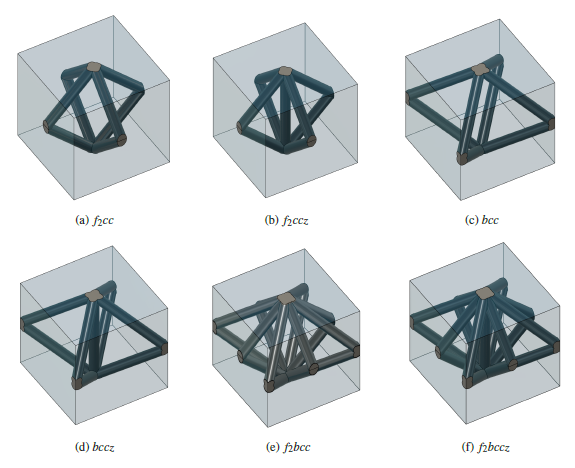
\includegraphics[width=0.7\linewidth]{figures/chapter_3/UnitCells.png}
    \caption{A selection of unit cells \cite{Piacquadio_Soika_Schirp_Schröder_Filippeschi_2023}}
    \label{fig:unit_cells}
\end{figure}

To simulate cellular structures, without having to mesh each cell, they can be treated as materials. For this, researchers have worked on homogenizing each type of cell to give effective material properties \cite{Piacquadio_Soika_Schirp_Schröder_Filippeschi_2023}\cite{Bühring_Soika_Schirp-Schoenen_Schröder_2022}. In structural mechanics, this involves determining the elastic modulus in each direction, whereas, in thermal problems, it involves determining the conductivity in each direction with an embedded PCM. The cells are considered porous media with porosity $\epsilon$. The porosity can be defined as the proportion of void volume to the total volume, or one minus the solid volume fraction $\mathcal{X}$ \cite{Piacquadio_Soika_Schirp_Schröder_Filippeschi_2023}, as shown in equation \ref{eq:porosity_definition}.
\begin{equation}
    \epsilon = 1 - \mathcal{X} = 1 - \frac{V_\text{solid}}{V_\text{total}}
    \label{eq:porosity_definition}
\end{equation} 

\subsection*{Structural Properties}
For the structural properties, only the matrix (the cell itself) is considered. This is because the selected phase change material, \emph{paraffin}, has a very low elastic modulus, relative to the material of the cell. Not only that but when the phase change material is in its liquid phase, then it provides no stiffness to the cells. For this thesis, the $bcc$ and $f_2 cc,z$ cells have been considered, but any other homogenized unit cell could be used instead. The properties were obtained from \cite{Bühring_Soika_Schirp-Schoenen_Schröder_2022}.

For the selected cells, only the Young's moduli in each direction are required. Young's modulus is non-linear for the unit cells. Figure \ref{fig:youngs_modulus_bcc_e1} shows the non-linear nature of Young's modulus. This will later have an impact on the topology optimization because the intermediate densities will have a different impact on how the structure grows.
\begin{figure}[ht]
    \centering
    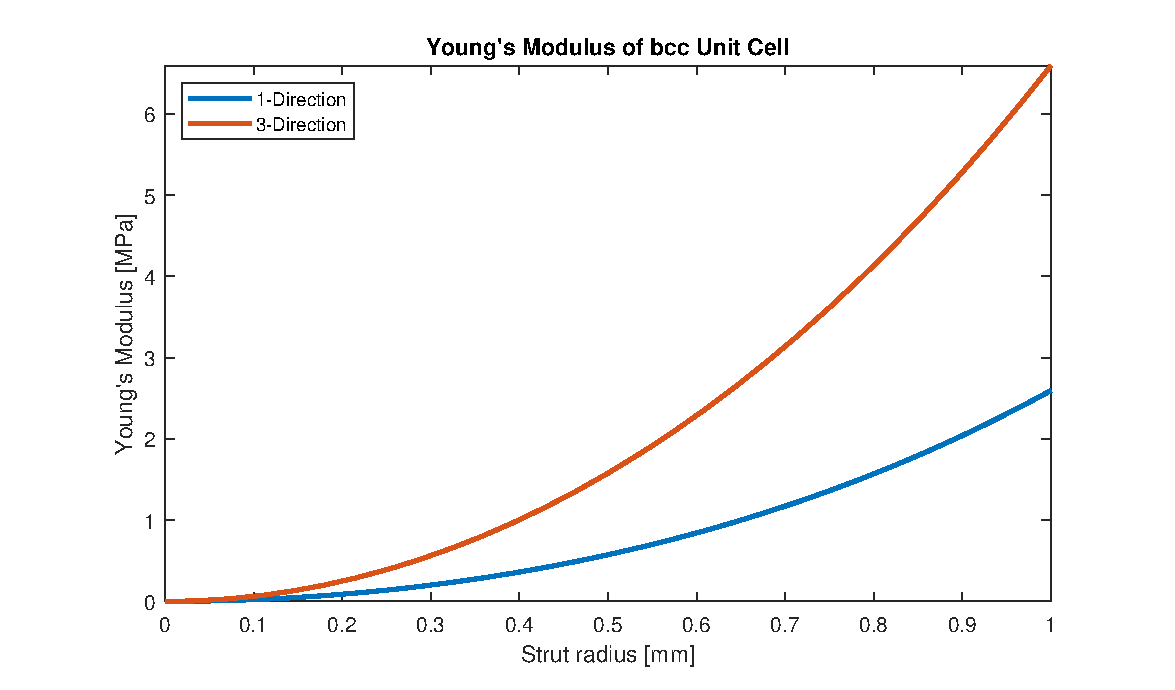
\includegraphics[width=0.9\linewidth]{figures/chapter_3/BCC_E1.eps}
    \caption{Young's Modulus of the BCC unit cell in each direction}
    \label{fig:youngs_modulus_bcc_e1}
\end{figure}


\subsection*{Thermal Properties}
The thermal properties of the unit cells are made up of both a highly conductive matrix (the cells themself), and a low-conductivity filler (phase change material). The cell properties are obtained from the master's thesis \cite{Piacquadio_Soika_Schirp_Schröder_Filippeschi_2023}. Again, this thesis only focuses on the $bcc$ and $f_2 cc,z$ cells, but any other homogenized unit cell could be used. The filler material is considered in these equations as it provides a non-negligible contribution to the thermal properties.

The required thermal properties that are needed are the effective thermal conductivity $k_{eff}$, the effective specific heat $c_{p, eff}$, and the effective latent heat $L_{eff}$. The specific heat and latent heat properties can be computed using the equations shown in equation \ref{eq:mixture_rules} which include the effective density $\rho_{eff}$ \cite{Piacquadio_Schirp-Schoenen_Mameli_Filippeschi_Schröder_2022}. Note that these equations all consider the porosity $\epsilon$.
\begin{subequations}
    \begin{equation}
        \rho_{eff} = \epsilon\rho_{\text{PCM}} + (1 - \epsilon)\rho_{\text{solid}}
    \end{equation}
    \begin{equation}
        c_{p, eff} = \epsilon\frac{\rho_\text{PCM}}{\rho_{eff}}c_{p,\text{PCM}} + (1 - \epsilon)\frac{\rho_\text{solid}}{\rho_{eff}}c_{p, \text{solid}} 
    \end{equation}
    \begin{equation}
        L_{eff} = \epsilon\frac{\rho_\text{PCM}}{\rho_{eff}}L_\text{PCM}
    \end{equation}
    \label{eq:mixture_rules}
\end{subequations}

Figure \ref{fig:thermal_properties} shows the properties of the $bcc$ unit cell as an example. Each of the properties is non-linear. Note that the effective latent heat is in terms of volume fraction, as this is important during the topology optimization. The specific heat curve is essentially a scaled version of the latent heat curve, so is not shown in the plots.
\begin{figure}[ht]
    \centering
    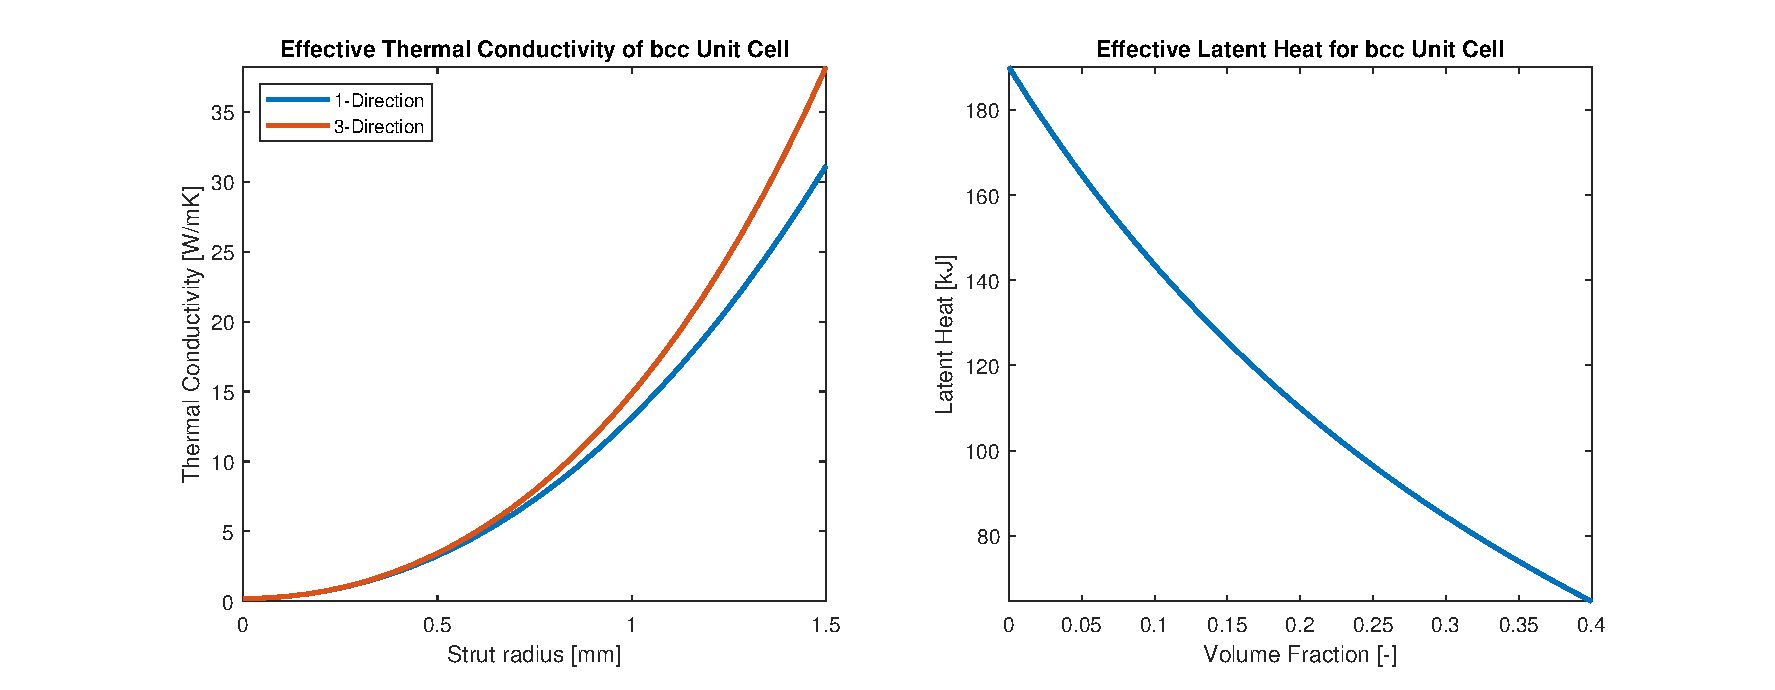
\includegraphics[width=0.95\linewidth]{figures/chapter_3/ThermalProperties.eps}
    \caption{Thermal properties of the $bcc$ unit cell}
    \label{fig:thermal_properties}
\end{figure}


\section{Latent Heat Energy Storage}
\label{chap:latent_heat_energy_storage}
Thermal energy storage is a method of storing heat in materials, either actively or passively, that can then be dissipated at a later time \cite{Cabeza_Martorell_Miró_Fernández_Barreneche_Cabeza_Fernández_Barreneche_2021}. One of the main uses currently is to assist the temporal and location mismatches between energy generation, and energy use. Thermal energy storage can also be used as a thermal management solution, where large amounts of heat may be generated irregularly, and can be dissipated passively over time.

A common thermal energy storage method is sensible heat energy storage. This method stores energy in a material without any phase change. The amount of sensible energy stored, $Q$, is expressed in equation \ref{eq:sensible_energy_storage} \cite{Cabeza_Martorell_Miró_Fernández_Barreneche_Cabeza_Fernández_Barreneche_2021}. Because this method involves no phase change, the best materials to select are those with a high specific heat $c_p$ and low cost. Materials such as water, oil and molten salts have been commonly used due to their availability and low cost. Note that the variable $m$ denotes the mass. Note that here $\Delta T = T - T_\text{ref}$, where $T_\text{ref}$ is the initial or ambient temperature.
\begin{equation}
    Q = m c_p \Delta T 
    \label{eq:sensible_energy_storage}
\end{equation}

In contrast to sensible heat energy storage, latent heat energy storage relies on the phase transition enthalpy $\Delta h$, or latent heat $L = \Delta h$, of a material to store vast amounts of energy for virtually no change in temperature \cite{Cabeza_Martorell_Miró_Fernández_Barreneche_Cabeza_Fernández_Barreneche_2021}. The total absorbed energy of the material can be expressed as shown in equation \ref{eq:total_sensible_energy}, which is the sum of sensible energy storage resulting in the solid and liquid phase, and the latent heat of melting. Latent heat energy storage materials are referred to as phase change materials. Note that the subscripts denote the solid phase $s$ or liquid phase $l$. Also note that $\Delta T_s = T_\text{melt} - T_\text{ref}$ and $\Delta T_f = T - T_\text{melt}$.
\begin{equation}
    Q = m c_{p,s}\Delta T_s + mL + m c_{p,l}\Delta T_l
    \label{eq:total_sensible_energy}
\end{equation}

Comparing the two methods, as shown in figure \ref{fig:sensible_vs_latent_storage}, the choice of energy storage method should depend on the application. When the temperature range is large, sensible energy storage can store much more energy, while in a narrow temperature range, latent heat energy storage is far superior. 
\begin{figure}[ht]
    \centering
    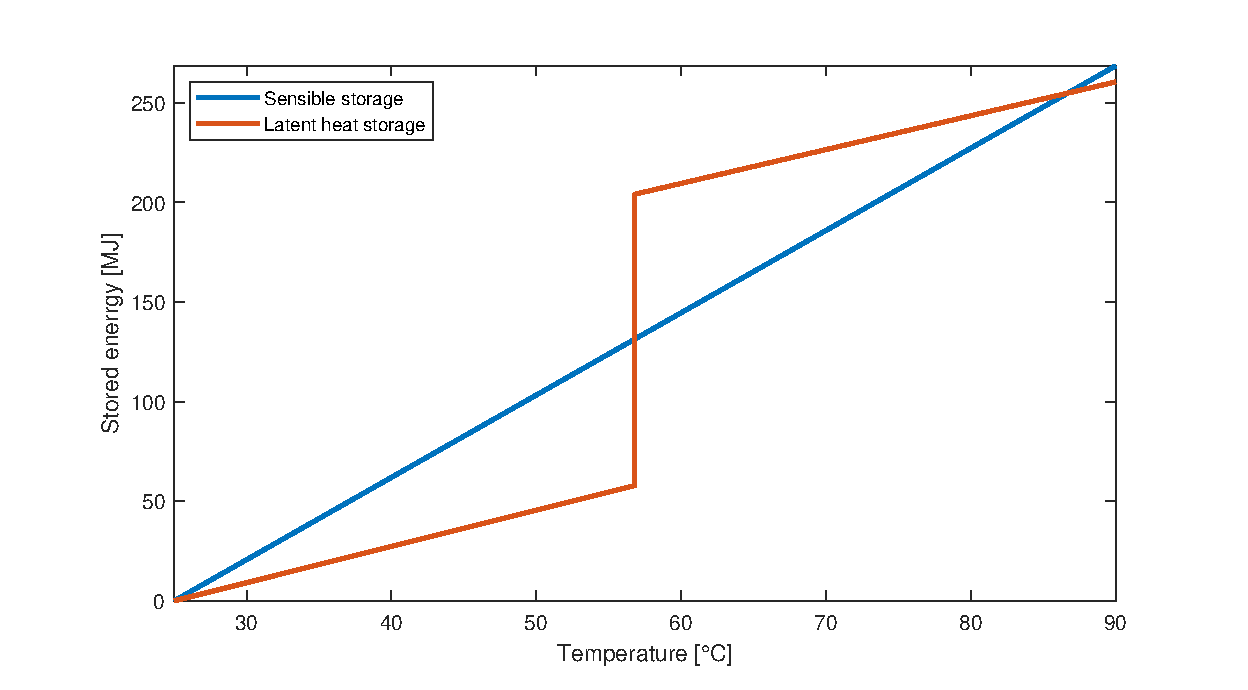
\includegraphics[width=0.7\linewidth]{figures/chapter_3/SensibleAndLatentStorage.eps}
    \caption{Sensible energy storage in water vs. the latent heat energy storage in paraffin}
    \label{fig:sensible_vs_latent_storage}
\end{figure}

\subsection*{Phase Change Materials}
The selection of phase change materials can be quite complex. The most important criteria are shown in table \ref{table:pcm_selection} \cite{Gadhave_Prabhune_Pathan_2020}. The most obvious selection criterion is the melting temperature of the material. This needs to be within the operating temperature, otherwise, it will simply act as a sensible heat storage medium. The next major selection criterion is the latent heat of the material. The higher, the more energy can be stored, and the longer the material remains around the melting temperature. Another very important property is the thermal conductivity. Having a low thermal conductivity would mean the temperature gradient in the domain could be quite high. This is not desirable when used in a cooling situation. 

The physical properties are also quite important to consider. If the phase change material is in a fixed volume, then the density change of the material could lead to very high pressures being sustained. It is for this reason that phase change materials are usually selected for solid-to-liquid phase change.
\begin{table}[ht]
    \centering
    \caption{Phase change material selection \cite{Gadhave_Prabhune_Pathan_2020}}
    \begin{tabular}{ c | c } 
        \hline
        \multirow{4}{*}{Thermal} & Melting temperature \\ & Latent heat \\ & Thermal conductivity \\ & Specific heat \\
        \hline
        \multirow{3}{*}{Physical} & High density \\ & Volume change \\ & Low vapour pressure \\
        \hline
        \multirow{3}{*}{Chemical} & Chemical stability \\ & Non-corrosiveness \\ & Non-flammability \\
        \hline
        \multirow{3}{*}{Economical} & Availability \\ & Cost \\ & Commercial viability \\
        \hline
    \end{tabular}
    \label{table:pcm_selection}
\end{table}

Some common phase change materials are shown in figure \ref{fig:pcm_selection}. A particularly good phase change material is water/ice, due to it having a high melting enthalpy and high availability. However, at ambient temperatures, the ice would have already melted, and therefore, only act as a sensible heat energy storage medium. Instead, paraffins have become a promising phase change material. Paraffins are organic materials that are a mixture of straight-chain n-alkanes \cite{Reza_Vakhshouri_2020}. By increasing the chain length, the melting temperature, as well as the latent heat increases \cite{Reza_Vakhshouri_2020}. This allows the material to be fine-tuned, to a degree, to the specific low-temperature use case. Of course, the other selection criteria also need to be considered.
\begin{figure}[ht]
    \centering
    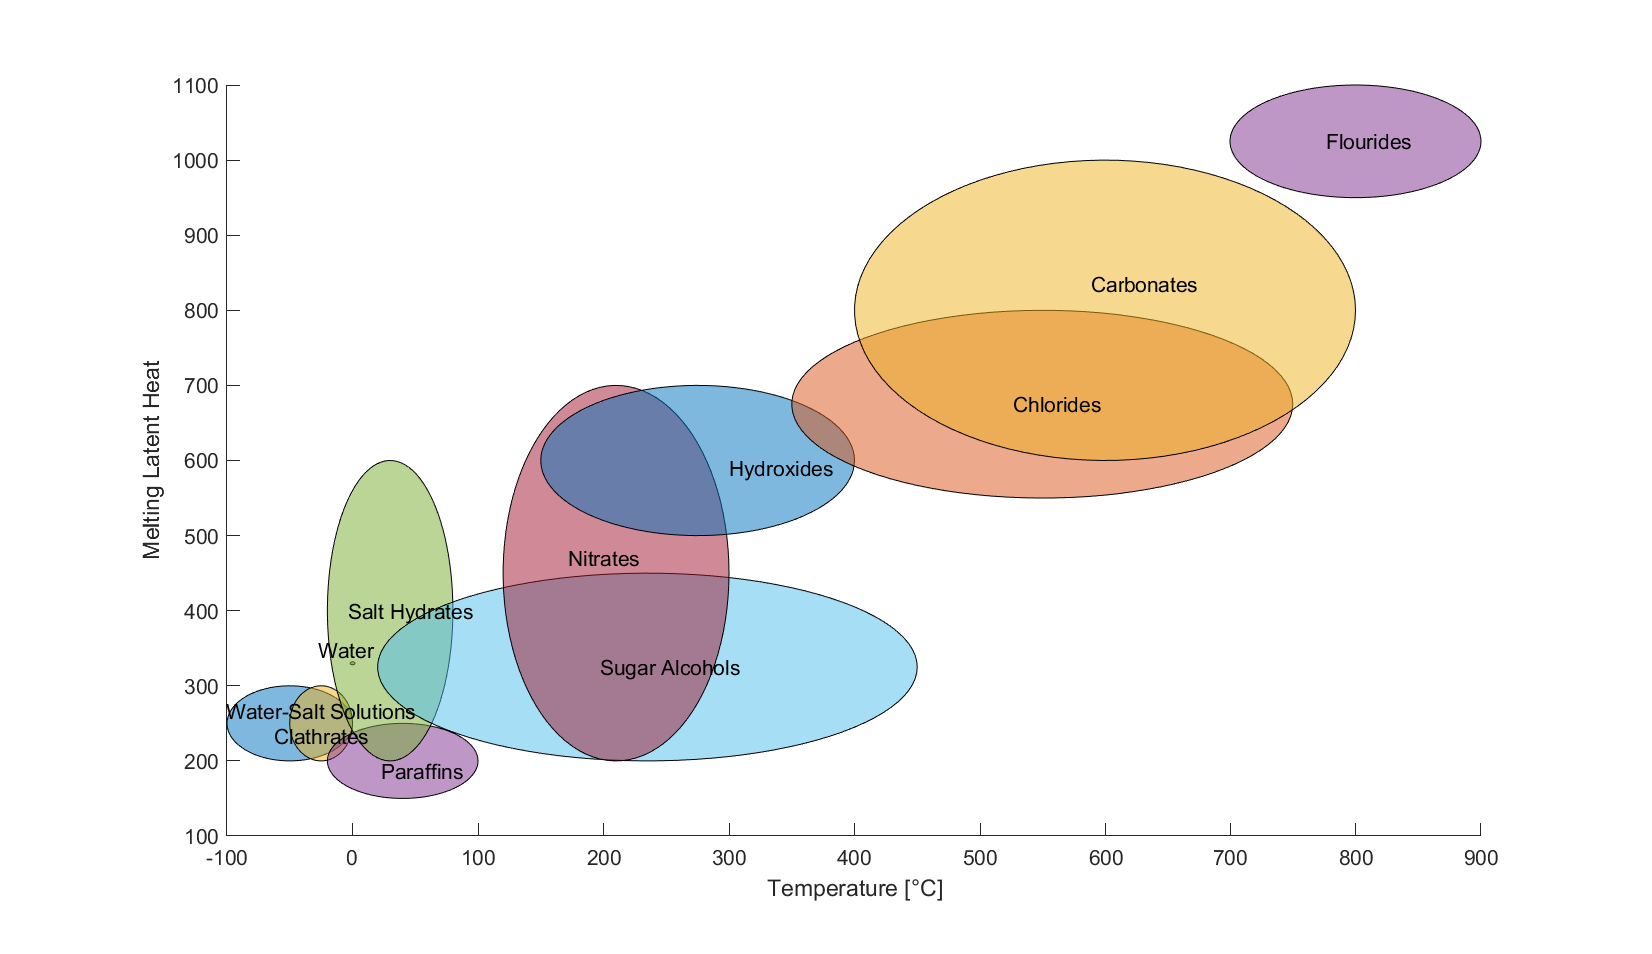
\includegraphics[width=0.8\linewidth]{figures/chapter_3/PCMs.eps}
    \caption{Phase change material selection chart \cite{Cabeza_Martorell_Miró_Fernández_Barreneche_Cabeza_Fernández_Barreneche_2021}}
    \label{fig:pcm_selection}
\end{figure}


\section{Topology Optimization}
\label{chap:topology_optimization}
Topology optimization is a shape optimization technique that is used to automatically design an ideal structure based on a set of boundary conditions. It works by distributing material throughout a domain only into the regions where it is required. In structural mechanics, this results in truss-like structures whereas in thermal problems, it results in organic tree-like structures. 
\begin{figure}[ht]
    \centering
    \begin{subfigure}[b]{0.49\linewidth}
        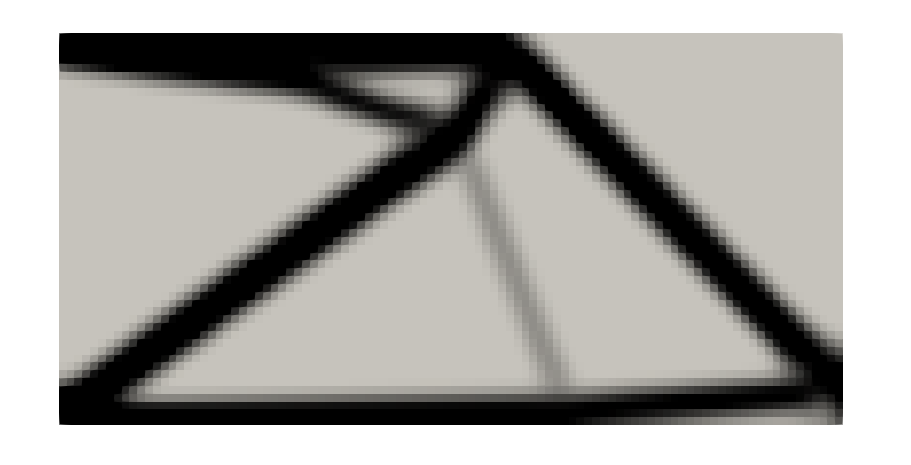
\includegraphics[width=\linewidth]{figures/chapter_3/SolidOpt.png}
        \caption{Solid isotropic material optimization}
    \end{subfigure}
    \begin{subfigure}[b]{0.49\linewidth}
        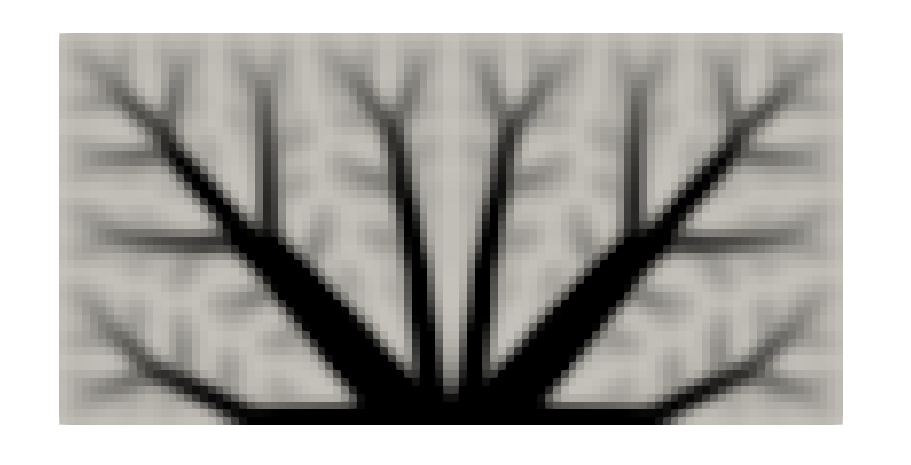
\includegraphics[width=\linewidth]{figures/chapter_3/ThermalOpt.png}
        \caption{Thermal isotropic material optimization}
    \end{subfigure}
    \caption{Examples of optimized domains for structural and thermal problems}
\end{figure}

To perform a topology optimization, the boundary conditions must be specified. The final volume $V$ of the structure should also be defined which is used to define how much material can be distributed. Lastly, some solid or void regions can also be defined which enforces full or empty regions in the domain. These may be desired for screw locations for example. Other than these quantities, the shape and connectivity of the structure are unknown \cite{Bendsøe_2004}.

\subsection*{Compliance Minimization using SIMP}
To optimize the domain, a function needs to be minimized (or maximized). The most common approach is to iteratively minimize the compliance, $c$, of the design, which in the context of a structural problem, maximizes the stiffness. Using the finite element method, the discrete form of this problem is given in equation \ref{eq:minimum_compliance_topopt} \cite{Bendsøe_2004} where $\mathbf{f}$ is the forcing array or right-hand side coming from the discretized system of equations, $\mathbf{u}$ is the vector of unknowns, $\mathbf{K}$ is the stiffness matrix coming from the system of equations and $D_e$ is the element material tensor that could be a conductivity or strain matrix. The compliance is essentially a measure of the objective because it relates the displacements or temperature at a boundary condition to the force or flux on that boundary. By minimizing compliance, the displacement or temperature is minimized on that boundary.
\begin{equation}
    \begin{alignedat}{2}
        &\min  \quad && c = \mathbf{f}^T \mathbf{u} \\
        &\text{s.t:} && \mathbf{K}(D_e)\mathbf{u}=\mathbf{f}
    \end{alignedat}
    \label{eq:minimum_compliance_topopt}
\end{equation}

One problem with this formulation is that it is non-differentiable due to the binary nature of materials. This restriction can be relaxed by introducing an interpolation function that smooths this transition. The most popular of which is the \emph{'Solid isotropic material with penalization (SIMP)'} \cite{Bendsøe_2004}, shown in equation \ref{eq:solid_iso_mat_pen}. In this equation, $D_0$ is the real material tensor, and $D_e$ is the penalized material tensor.
\begin{equation}
    D_e(x) = \rho(x)^p D_0, \quad p > 1
    \label{eq:solid_iso_mat_pen}
\end{equation}

Equation \ref{eq:solid_iso_mat_pen} introduces the element relative density $\rho(x) \in [0,1]$ which interpolates between the material being present ($\rho=1$), or void ($\rho=0$). The equation also introduces the penalization parameter $p$ which is used to penalize intermediate densities. By doing so, it ensures that the intermediate densities are undesirable, and forces them to become either solid or void \cite{Bendsøe_2004}. Usually, $p\geq 3$ to ensure the intermediate densities are penalized enough. With that, equation \ref{eq:minimum_compliance_topopt} can be slightly reformulated as given in equation \ref{eq:top_opt_simp}. The second constraint is the volume constraint which ensures the final volume is less than or equal to the user-defined maximum volume.
\begin{equation}
    \begin{alignedat}{2}
        &\min \quad &&c(\rho(\mathbf{x}))=\mathbf{f}^T\mathbf{u} \\
        & s.t \quad &&\mathbf{K}(D_e(\mathbf{x}))\mathbf{u}=\mathbf{f} \\ 
        & && \int_\Omega \rho(x) \ d\Omega \leq V
    \end{alignedat}
    \label{eq:top_opt_simp}
\end{equation}

\subsubsection*{\emph{Complications}}
While this formulation can obtain a structure, many complications must be dealt with. The main complication is the so-called \emph{'checkerboard'} problem \cite{Bendsøe_2004}. These are a result of poor numerical modeling that overestimates the stiffness, similar to problems that occur in the pressure field in Stokes flow problems using FEM \cite{Bendsøe_2004}. As a result of the checkerboard pattern, the optimized structure is non-physical. To resolve this problem, filtering can be used. Many filters have been proposed, such as those investigated by Sigmund \cite{Sigmund_2007}. Of those proposed, the so-called density or sensitivity filters are the most popular for their ease of implementation and efficiency \cite{Sigmund_2007}. These act like low-pass filters which essentially blurs the sensitivities in a local region. Equation \ref{eq:sensitivity_filter} shows the form of a sensitivity filter \cite{Sigmund_1997} and equation \ref{eq:density_filter} shows the form of a density filter \cite{Bruns_Tortorelli_2001}. Each uses a filter matrix, such as the one shown in equation \ref{eq:filter_matrix} with filter radius $r$. Using the suggested filter matrices also has the effect of making the results mesh-independent.
\begin{subequations}
    \begin{equation}
        H_{ij} = \max(r-\lVert x_i - x_j \rVert, 0)
        \label{eq:filter_matrix}
    \end{equation}
    \begin{equation}
        \widetilde{\frac{\partial c_i}{\partial \rho_e}} = \frac{1}{\rho_i \sum_{j=1}^N H_{ij}} \ \sum_{j=1}^N H_{ij}\rho_j \frac{\partial c_i}{\partial \rho_j}
        \label{eq:sensitivity_filter}
    \end{equation}
    \begin{equation}
        \widetilde{\rho_i} = \frac{\sum_{j=1}^N H_{ij}v_j\rho_j}{\sum_{j=1}^N H_{ij}v_j}
        \label{eq:density_filter}
    \end{equation}
\end{subequations}

Figure \ref{fig:no_filtering} shows an optimized structure with no filtering. It shows checkerboarding in the top middle area, as well as struts with elements that only join at one node. Such a structure could not be manufactured due to these voids.
\begin{figure}[ht]
    \centering
    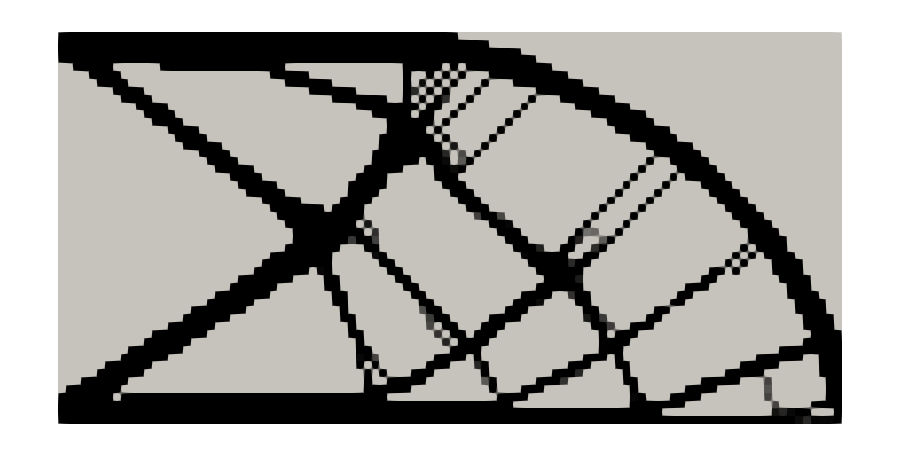
\includegraphics[width=0.8\linewidth]{figures/chapter_3/OptNoFilter.png}
    \caption{Checkerboard pattern and non-physical regions resulting from no filter}
    \label{fig:no_filtering}
\end{figure}

Another issue with topology optimization is that many local minima can be obtained for the same given set of boundary conditions \cite{Bendsøe_2004}. These can be found by changing the initial structure, or by using different penalization parameters. Some methods have been used to overcome this problem, but one simple approach is to gradually increase the penalization parameter from 1 to the desired value. Another method is to start with a large filter radius, and gradually decrease it \cite{Bendsøe_2004}.

\subsubsection*{\emph{Update Criterion}}
The final ingredient required to perform a topology optimization is to incrementally update the element's relative densities until a converged structure is obtained. The method of moving asymptotes has been used for updating the design variables \cite{Svanberg_1987} as well as the so-called \emph{'optimality criteria method'} \cite{Bendsøe_2004}. For this thesis, the optimality criteria method as well as the generalized optimality criteria method, proposed by Kim, et al., 2021 \cite{Kim_Dong_Weinberg_Dalidd_2021} has been adopted.

Recall that constrained optimization has been discussed in chapter \ref{chap:methods_for_optimization} where the idea of Lagrange multipliers was introduced. A Lagrangian can be constructed for a topology optimization problem as shown in equation \ref{eq:top_opt_lagrangian} \cite{Bendsøe_2004}. Note that $f$ is the volume fraction and $V_0$ is the total volume of the domain. This is equal to the user-defined final volume. For simplicity, $\mathbf{x}$ will be used in place of $\rho(\mathbf{x})$.
\begin{equation}
    \begin{split}
        \mathcal{L}(\mathbf{x},\lambda) &= c(\mathbf{x}) + \lambda(V(\mathbf{x}) - fV_0) \\
        \text{where: } V(\mathbf{x}) &= \int_\Omega\rho(\mathbf{x}) \ d\Omega
    \end{split}
    \label{eq:top_opt_lagrangian}
\end{equation}

A critical point is found when the following conditions in equation \ref{eq:top_opt_critical_cond} are met.
\begin{equation}
    \begin{split}
        \frac{\partial \mathcal{L}}{\partial \mathbf{x}} = \frac{\partial c(\mathbf{x})}{\partial \mathbf{x}} + \lambda\frac{\partial V(\mathbf{x})}{\partial \mathbf{x}} = 0\\
        \frac{\partial \mathcal{L}}{\partial \lambda} = V(\mathbf{x}) - fV_0 = 0
    \end{split}
    \label{eq:top_opt_critical_cond}
\end{equation}

To determine the Lagrange multiplier $\lambda$, the first constraint can be rearranged as shown in equation \ref{eq:scale_factor} for each element. This variable is called the scale factor, and an optimum is reached when it is equal to one. The optimal Lagrange multiplier can be found using bisection or similar methods.
\begin{equation}
    B_e = -\frac{\frac{\partial c(\mathbf{x})}{\partial x_e}}{\lambda\frac{\partial V(\mathbf{x})}{\partial x_e}}
    \label{eq:scale_factor}
\end{equation}

With that, each element can have its relative density updated according to equation \ref{eq:o_c_m}. This approach limits how much each element can be updated by controlling the move $m$ parameter. The value $\eta$, often set to 0.5, is used to control how quickly and stable the solution can converge \cite{Bendsøe_2004}. 
\begin{equation}
    \rho_{k+1} = \begin{cases}
        \max{((1 - m)\rho_k, \ \rho_{min})} & \text{if} \ \rho_kB_k^\eta \leq \max{((1 - m)\rho_k, \ \rho_{min})} \\
        \min{((1 + m)\rho_k, \ \rho_{max})} & \text{if} \ \rho_kB_k^\eta \geq \max{((1 + m)\rho_k, \ \rho_{max})} \\
        \rho_kB_k^\eta & \text{otherwise}
    \end{cases}
    \label{eq:o_c_m}
\end{equation}

The generalized optimality criteria method (GOCM) extends the standard version by allowing multiple inequality constraints with improved computational efficiency \cite{Kim_Dong_Weinberg_Dalidd_2021}. A more general version of the Lagrangian is given below in equation \ref{eq:general_opt_lagrangian}, which also includes a slack variable. This variable is non-zero when the constraint is inactive.
\begin{equation}
    \mathcal{L}(\mathbf{x},\lambda,\mathbf{s}) = c(\mathbf{x}) + \sum_{i=1}^N\lambda_i(g_i(\mathbf{x})+s_i^2)
    \label{eq:general_opt_lagrangian}
\end{equation}

A critical point is found when the gradient of the Lagrangian is zero. This results in equation \ref{eq:general_opt_critical_condition} \cite{Kim_Dong_Weinberg_Dalidd_2021}. Because of the third condition, only the active constraints need to be considered \cite{Kim_Dong_Weinberg_Dalidd_2021}.
\begin{equation}
    \begin{split}
        & \nabla_\mathbf{x}c(\mathbf{x}) + \sum_{i=1}^N\lambda_i\nabla_\mathbf{x}g_i = 0 \\
        & g_i(\mathbf{x})+s_i^2 = 0, \  i\in [1,N] \\
        & \nabla_i s_i = 0
    \end{split}
    \label{eq:general_opt_critical_condition}
\end{equation}

One of the ideas proposed by Kim, et al., the Lagrange multipliers don't need to be satisfied for every iteration. As a result, very little computational resources are needed for each iteration to find the Lagrange multipliers. Instead, they are updated each iteration until convergence \cite{Kim_Dong_Weinberg_Dalidd_2021}. Patnaik et al., \cite{Patnaik_Guptill_Berke_1995} proposed a few options for this. Two of which are given in equation \ref{eq:linear_lagrange_update}. The third option is proposed by Kim et al., \cite{Kim_Dong_Weinberg_Dalidd_2021} which aims to control how quickly the Lagrange multiplier is found. The relative densities can then be updated according to equation \ref{eq:o_c_m}
\begin{equation}
    \begin{alignedat}{2}
        \lambda_i^{k+1} &= \lambda_i^k(1+\alpha^kp_0g_i) \quad && \text{Linear form} \\
        \lambda_i^{k+1} &= \lambda_i^k(g_i)^{\alpha^kp_0} \quad && \text{Exponential form} \\
        \lambda_i^{k+1} &= \lambda_i^k(1+p_0(g_i^k + \Delta g_i^k)) \quad && \text{Kim et al., (2023)}
    \end{alignedat}
    \label{eq:linear_lagrange_update}
\end{equation}   

\subsection*{Structural Optimization}
Structural topology optimization is a very useful tool in engineering. It is capable of giving a designer a rough idea of how to design a structure by maximizing its stiffness, or by minimizing its stress. The goal function, as shown in equation \ref{eq:structural_compliance} is to minimize the compliance, which has the effect of maximizing stiffness.
\begin{equation}
    \begin{alignedat}{2}
        &\min \quad &&c(\rho) = \mathbf{u}^T\mathbf{f} \\
        & s.t \quad &&\mathbf{K}(D_e(\mathbf{x}))\mathbf{u}=\mathbf{f} \\ 
        & && \int_\Omega \rho(x) \ d\Omega \leq V
    \end{alignedat}
    \label{eq:structural_compliance}
\end{equation}

The gradient of the compliance, as given by Bendsøe, et al., 2004 \cite{Bendsøe_2004} is shown, without derivation, in equation \ref{eq:structural_compliance_gradient}. Note that this only considers the theory of small displacements. Non-linear problems are more complex but are not required for this thesis.
\begin{equation}
    \frac{\partial c}{\partial \rho_e} = -\mathbf{u}^T\frac{\partial\mathbf{K_e}}{\partial\rho_e}\mathbf{u}
    \label{eq:structural_compliance_gradient}
\end{equation}

\subsection*{Thermal Optimization}
Thermal topology optimization has become a well-researched topic with many methods now existing \cite{Bendsøe_2004} \cite{Alexandersen_Sigmund_Aage_2016}. Thermal compliance as shown in equation \ref{eq:thermal_compliance}, which is analogous to structural compliance, is the goal function being minimized. By minimizing the thermal compliance, the temperature at the heat flux boundary is minimized. 
\begin{equation}
    \begin{alignedat}{2}
        &\min \quad &&c(\rho) = \mathbf{T}^T\mathbf{f} \\
        & s.t \quad &&\mathbf{K}(k_e(\mathbf{x}))\mathbf{T}=\mathbf{f} \\ 
        & && \int_\Omega \rho(x) \ d\Omega \leq V
    \end{alignedat}
    \label{eq:thermal_compliance}
\end{equation}

The gradient of the compliance, as given by Joo, et al., 2017 \cite{Joo_Lee_Kim_2017} is shown, without derivation, in equation \ref{eq:thermal_compliance_gradient}. They found the derivative of the convection matrix $\mathbf{K}_h$ to be negligible, and the derivative of the forcing array is known to be zero. As a result, only the conductivity matrix $\mathbf{K}_c$ has an impact on the total gradient.
\begin{equation}
    \frac{\partial c}{\partial \rho_e} = 2\mathbf{T}^T\frac{\partial\mathbf{f}_e}{\partial\rho_e}-\mathbf{T}^T\left( \frac{\partial\mathbf{K}_{e,h}}{\partial\rho_e} + \frac{\partial\mathbf{K}_{e,c}}{\partial\rho_e} \right)\mathbf{T} = -\mathbf{T}^T\frac{\partial\mathbf{K}_{e,c}}{\partial\rho_e}\mathbf{T}
    \label{eq:thermal_compliance_gradient}
\end{equation}

In this thesis, domains are considered to be purely conductive. In spacecraft systems, the force of gravity is absent, so no natural convection will occur. This means that the convection matrix is irrelevant, and no assumptions need to be made for it. Of course, this is not the case for phase change domains, where latent heat effects are present, but the case for pure conduction will be considered as a highly simplified phase change domain.

\subsection*{Optimization of Lattice Structures}
Optimization of lattice structures is essentially topology optimization considering orthotropic material properties. During the optimization loop, the orientation of the cells is considered to achieve greater stiffness. This can be achieved by aligning the unit cells along the principal stress axes \cite{Groen_Sigmund_2017}. A rotation matrix such as the one in equation \ref{eq:rotation_matrix} can be used to rotate the material tensor, as shown in equation \ref{eq:rotated_material_tensor}.
\begin{subequations}
    \begin{equation}
        \mathbf{C}(x,\theta) = \mathbf{R}^T(\theta) \mathbf{C}(x) \mathbf{R}(\theta)
        \label{eq:rotated_material_tensor}
    \end{equation}
    \begin{equation}
        \mathbf{R}(\theta) = \begin{bmatrix}
            \cos \theta & -\sin \theta \\
            \sin \theta & \cos \theta
            \label{eq:rotation_matrix}
        \end{bmatrix}
    \end{equation}
\end{subequations}

The optimization loop is similar to a typical topology optimization, but during each iteration, the principal stresses need to be determined as well as their angle. The material tensor can then be rotated and recomputed until the change in angle is below a tolerance. The principle axis can be computed using equation \ref{eq:principal_axis}.
\begin{equation}
\tan(2\theta_p) = \frac{2\tau_{xy}}{\sigma_x - \sigma_y}
\label{eq:principal_axis}
\end{equation}

In this thesis, this method has not been implemented. It had been decided early on that the added complication of considering the cell orientation was not as important as the multi-functional component of the thesis. A simple substep could be implemented, however, in future work.

After an optimal structure has been generated, it is de-homogenized as a post-processing step. Many methods have been proposed for this \cite{Groen_Sigmund_2017} \cite{Larsen_Sigmund_Groen_2018} \cite{Fernandes_Tamijani_2021}. The de-homogenization step is required to return the finite element mesh into a meaningful lattice representation. The cited examples, however, are quite complex. In this thesis, the cell size was decided to be kept constant. That combined with no cell alignment means that the mesh can be projected back onto a lattice mesh, and some methodology can be determined for averaging the element relative densities over each unit cell. This is beyond the scope of this thesis, but a simple example has been implemented for visualization purposes in future chapters.

\subsection*{Multi-functional Topology Optimization}
Topology optimization has been successfully applied to multi-functional problems. Many methods have evolved for optimizing lattice unit cells \cite{Zhang_Ye_Wei_Tao_Luo_2021} \cite{Imediegwu_Murphy_Hewson_Santer_2021} \cite{Challis_Roberts_Wilkins_2008}. This thesis focuses on optimizing a domain given an already homogenized unit cell, so a similar approach to Pejman and Najafi, \cite{Pejman_Najafi_2023} has been adopted. Takezawa, et al., \cite{Takezawa_Yoon_Jeong_Kobashi_Kitamura_2014} also developed a method for structural optimization using stress and conduction constraints, where some ideas have also been adopted.

To generate a Pareto front, the weight method has been used, similar to how Challis, et al., \cite{Challis_Roberts_Wilkins_2008} described. Here, the objective function is to minimize equation \ref{eq:weight_method_compliance}, where $w_i$ are weights that sum to one of the relative importance of each separate function $c_i$.
\begin{equation}
    J = - \left(w_1c_1 + w_2c_2\right)
    \label{eq:weight_method_compliance}
\end{equation}

Pejman and Najafi \cite{Pejman_Najafi_2023} proposed a method to obtain a Pareto front by first computing the single field problems to determine the bounds. The compliance of the single functions can then be normalized, and a Pareto front can be generated by incrementing the weights from $0$ to $1$. This methodology has been adapted for this thesis in chapter \ref{chap:multi-functional_optimization}. The gradient of the objective function ends up being a sum of the gradients of the single functional components with a weight on each.

Figure \ref{fig:pejman_najafi} shows each step proposed by Pejman and Najafi \cite{Pejman_Najafi_2023}. In part A, the bounds of the Pareto front are determined by the single functional components. The maximum of the opposite function occurs when the other function is a minimum. Part B shows the Pareto front being normalized. Points are then evenly spaced along the Pareto front to obtain intermediate points in part C. 
\begin{figure}[ht]
    \centering
    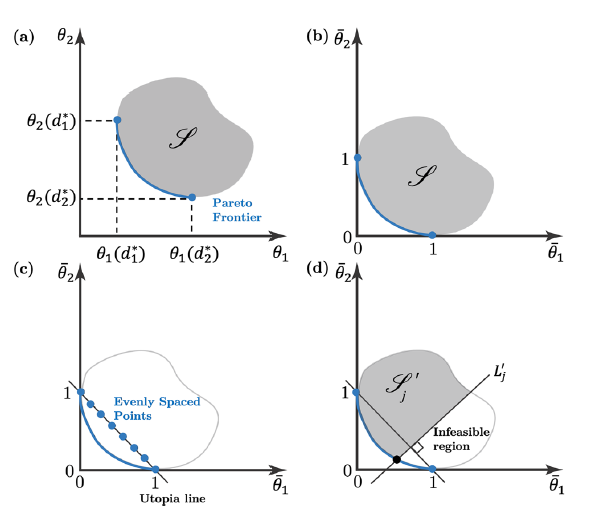
\includegraphics[width=0.6\linewidth]{figures/chapter_3/MultifunctionalSubsteps.png}
    \caption{Illustrated steps proposed by Pejman and Najafi, 2023 \cite{Pejman_Najafi_2023}}
    \label{fig:pejman_najafi}
\end{figure}


\section{Numerical Methods for Phase Change Problems}
In chapter \ref{chap:stefan_problem}, the Stefan problem was briefly introduced. In this section, some numerical methods will be introduced which are capable of solving phase-change problems. Many methods exist to solve phase change problems such as those discussed by Zeneli et al. \cite{Zeneli_Nikolopoulos_Karellas_Nikolopoulos_2021}

Front-tracking methods for instance explicitly track the phase transition front \cite{Dehghan_Najafi_2016}. These methods first compute the location of the boundary and then solve the heat equation and other required equations ensuring the proper boundary conditions are satisfied. They generally use an adaptive or a deforming mesh to try to capture the phase transition front. This method has been successfully applied to the finite element method \cite{Zhao_Heinrich_2001}. This method will not be discussed further, as having an adaptive or deforming mesh makes the topology optimization module extremely difficult to implement.

Front-fixing methods are similar to front-tracking methods. They explicitly track the phase transition front, but also fix the grid to the front. Due to this, this method has a high degree of complexity and is recommended for simple geometries \cite{Zeneli_Nikolopoulos_Karellas_Nikolopoulos_2021}. This method will also not be discussed further, as it makes the topology optimization module very complex to implement.

The final, and most common family of methods are the fixed-domain methods. These methods are also much simpler to implement, and still have a high degree of accuracy, even without having a mesh that closely tracks the phase transition front. One of the most common methods is the enthalpy method \cite{Voller_Cross_Markatos_1987}. In this method, the phase transition front is indirectly tracked by solving a modified heat equation in terms of enthalpy \ref{eq:enthalpy_method}. This method could be easily adapted to topology optimization as it uses a fixed mesh. However, in this thesis, the apparent heat capacity method, which is yet to be discussed, was selected for its temperature formulation.
\begin{equation}
    \frac{\partial H}{\partial t} = \alpha_H\nabla^2H=\alpha c_p \nabla^2 T
    \label{eq:enthalpy_method}
\end{equation}

The level set method has also successfully been used to capture phase-change problems \cite{Osher_Sethian_1988}. In the level-set method, the transition boundary is tracked using a signed distance function, and described by equation \ref{eq:level_set_method}. Where the function is zero, is where the phase transition boundary lies. The level set function changes in time by some velocity, which is governed by the Stefan condition.
\begin{equation}
    \varphi =\begin{cases}
        -d, \quad &\text{Solid} \\ 0, \quad &\text{Interface} \\ d, \quad &\text{Liquid}
    \end{cases}
    \label{eq:level_set_method}
\end{equation}

\subsection*{Heat Capacity Method}
The heat capacity method is similar to the enthalpy method in that it solves a slightly modified heat equation. However, it is formulated directly around the temperature making it easy to implement. The heat-capacity method (as well as other fixed domain methods) makes use of a so-called "mushy zone" which relaxes the jump condition at the phase transition boundary. Figure \ref{fig:mushy_zone} illustrates how the mushy-zone can be modeled with different functions. The plot describes the phase fraction evolution, where zero represents a solid and one represents a liquid. By taking the derivative of these functions, a Dirac-delta function is approximated.
\begin{figure}[ht]
    \centering
    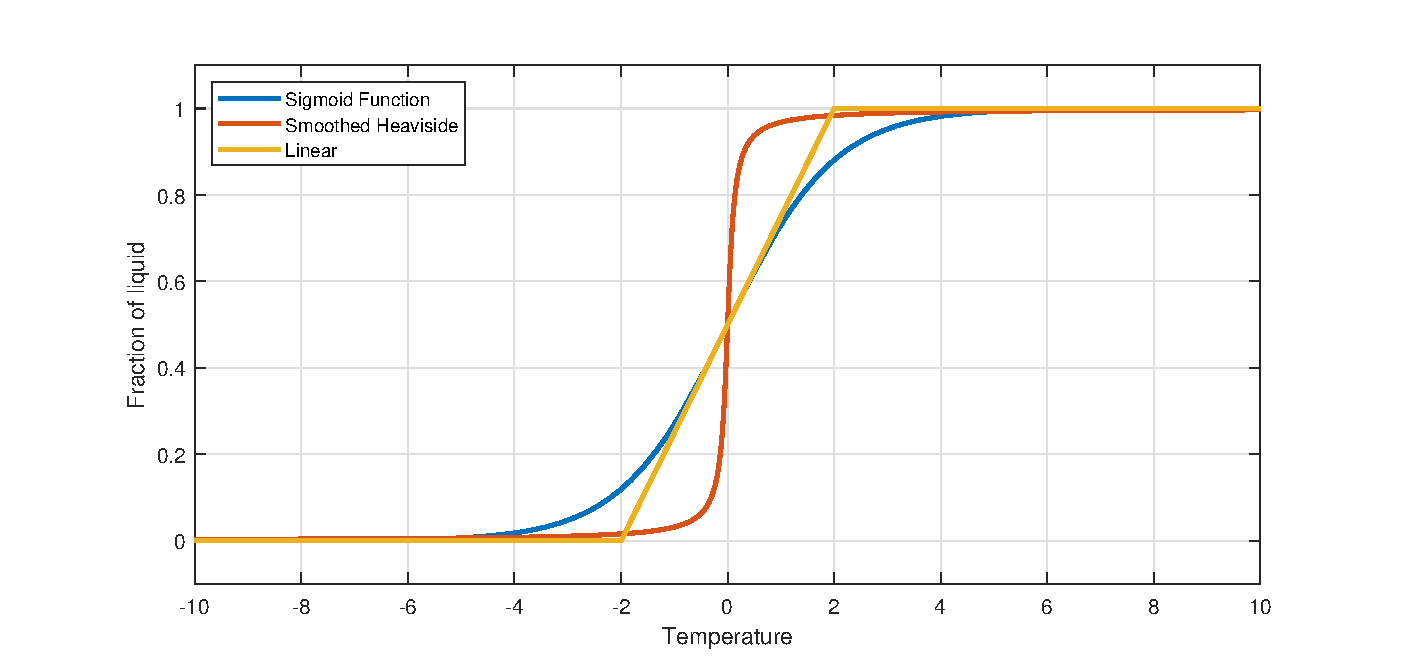
\includegraphics[width=0.9\linewidth]{figures/chapter_3/MushyZone.eps}
    \caption{Various phase transition functions}
    \label{fig:mushy_zone}
\end{figure}

The apparent heat capacity method \cite{Comini_DelGuidice_Lewis_Zienkiewicz_1974} has been utilized for this thesis. The heat capacity method works by having the heat capacity, as well as other material properties, be temperature-dependant variables, as shown in figure \ref{fig:material_properties_phase_change}. Across the mushy zone, the heat capacity jumps as a result of the latent heat of melting. The material properties can be smoothed to improve the solver's stability using the suggested functions in figure \ref{fig:mushy_zone}. The sigmoid function has been used with particular success \cite{Yang_He_2010}.
\begin{figure}[ht]
    \centering
    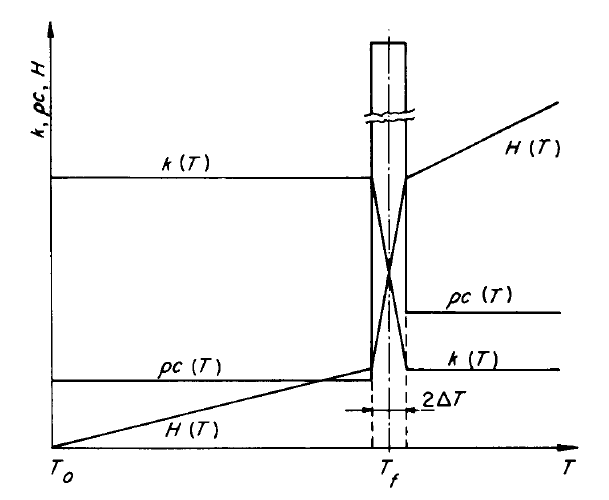
\includegraphics[width=0.6\linewidth]{figures/chapter_3/MaterialPropertiesOverPhaseChange.png}
    \caption{Material properties variation over phase change boundary \cite{Comini_DelGuidice_Lewis_Zienkiewicz_1974}}
    \label{fig:material_properties_phase_change}
\end{figure} 

In the apparent heat capacity method, the time-dependent heat equation shown in equation \ref{eq:time_dependant_heat_equation} is solved. Where $\rho$ is the material density, $c_{app}$ is the apparent heat capacity, and $k$ is the thermal conductivity. Some materials, such as paraffin wax have a relatively constant thermal conductivity, so for this analysis, it will be considered constant.
\begin{equation}
    \rho c_{app}(T) \frac{\partial T}{\partial t} = \nabla \cdot (k \nabla T) + q
    \label{eq:time_dependant_heat_equation}
\end{equation}

The heat capacity is defined by $c_{app}=dU/dT$ for a constant volume process, where $U$ is the internal energy. In this case, the specific internal energy $u$ is a sum of the heat capacity $c_p$ and latent heat $L$ effects \cite{Nallathambi_Specht_Bertram_2009}, as shown in equation \ref{eq:apparent_heat_capacity}.
\begin{equation}
    u = \int_{T_{ref}}^T c_p dT + L f_p
    \label{eq:apparent_heat_capacity}
\end{equation}

Equation \ref{eq:apparent_heat_capacity} introduces the phase fraction $f_p$ which can be defined in various ways, as figure \ref{fig:mushy_zone} shows. Some equations are given below in equation \ref{eq:mushy_zone}. The phase fraction ranges from zero to one and is used to track how much a material point has melted. In the equations below, the variable $a$ can control how tight the phase transition is.
\begin{subequations}
    \begin{equation}
        f_p(T) = \frac{1}{1+e^{-a(T-T_m)}}, \quad \text{Sigmoid Function}
    \end{equation}
    \begin{equation}
        f_p(T) = \lim_{a\to 0} \ \frac{1}{\pi}\tan^{-1}\left(\frac{T-T_m}{a}\right) + \frac{1}{2}, \quad \text{Smooth Heaviside}
    \end{equation}
    \begin{equation}
        f_p(T) = \begin{cases}
            0, \quad &\text{In solid phase} \\
            \frac{1}{2\Delta T}(T-T_m), &\text{In mushy zone} \\
            1, \quad &\text{In liquid phase}
        \end{cases}, \quad \text{Linear Function}
    \end{equation}
    \label{eq:mushy_zone}
\end{subequations}

Substituting the apparent heat capacity into the heat equation, the continuous description of the problem is described as shown in equation \ref{eq:continuous_phase_change_heat} \cite{Nallathambi_Specht_Bertram_2009}. In this equation, the latent heat effects are only present when the phase fraction is in the mushy zone ($0<f_p<1$). This equation is also clearly non-linear and can be severely non-linear when the latent heat effects are large, and the mushy zone is small.
\begin{equation}
    \rho\left (c_p+L\frac{\partial f_p}{\partial T} \right )\frac{\partial T}{\partial t} = k\nabla^2T + f
    \label{eq:continuous_phase_change_heat}
\end{equation}

After discretization, a discrete system of equations can be found. Equation \ref{eq:discrete_phase_change} uses the derivation by Celentano et al. \cite{Celentano_Oñate_Oller_1994} and equation \ref{eq:matrix_phase_change} gives the finite element matrices. Note that $\dot{\mathbf{L}} = \mathbf{L}^{n+1}-\mathbf{L}^n$.
\begin{subequations}
    \begin{equation}
        \mathbf{K}T + \mathbf{C}\dot{T} + \dot{\mathbf{L}} = \mathbf{F}
        \label{eq:discrete_phase_change}
    \end{equation}
    \begin{equation}
        \begin{split}
            \mathbf{K}^e&=\int_{\Omega^e}(\nabla \text{N})^T  k  \nabla \text{N} \ d\Omega^e + \int_{\Gamma}h\text{N}\text{N}^Td \ \Gamma \\
            \mathbf{C}^e&=\int_{\Omega^e}\rho c_p \text{N}\text{N}^T \ d\Omega^e \\
            \mathbf{L}^e&=\int_{\Omega^e} \text{N}\rho L f_p \ d\Omega^e \\
            \mathbf{F}^e&=\int_{\Omega^e} \text{N}\rho b \ d\Omega^e + \int_{\Gamma} \text{N}hT_{\infty} \ d\Gamma
        \end{split}
        \label{eq:matrix_phase_change}
    \end{equation}
\end{subequations}

Using backward Euler, the equation can be rewritten in the residual form shown in equation \ref{eq:residual_form_phase_change}. Taking the derivative of this gives the Jacobian shown in equation \ref{eq:jacobian_phase_change}. Note that the subscript $i$ denotes an iteration index of an iterative scheme such as Newton's method.
\begin{subequations}
    \begin{equation}
        \mathbf{R}(T^{n+1}_i)=\mathbf{F}\Delta t + \mathbf{C}T^n-(\mathbf{L}^{n+1}_i-\mathbf{L}^n)-(\mathbf{C}+\mathbf{K}\Delta t)T^{n+1}_i
        \label{eq:residual_form_phase_change}
    \end{equation}
    \begin{equation}
        \mathbf{J}(T^{n+1}_i)=-\frac{\partial \mathbf{R}}{\partial T}\Big|_i^{n+1}=\mathbf{K}\Delta t + \mathbf{C} + \frac{\partial \mathbf{L}}{\partial T}\Big|_i^{n+1}
        \label{eq:jacobian_phase_change}
    \end{equation}
\end{subequations}

An iterative scheme can then be used to determine the temperature. First, the descent direction is computed using equation \ref{eq:newton_iteration_pc}.
\begin{equation}
    \Delta T = [\mathbf{J}(T_i^{n+1})]^{-1}\mathbf{R}(T_i^{n+1})
    \label{eq:newton_iteration_pc}
\end{equation}

The descent direction can then be used in an iterative scheme such as Newton's method ($\alpha = 1$), damped Newton's method ($0<\alpha<1$), or a line search to determine a step-size $\alpha$.
\begin{equation}
    T_{i+1}^{n+1} = T_{i}^{n+1} + \alpha\Delta T
\end{equation}

\subsection*{Effective Heat Capacity Method}
The effective heat capacity method \cite{Poirier_Salcudean_1988} is another heat capacity method worth mentioning that considers the temperature distribution between the nodes in a mesh. It resolves the issue that a narrow mushy zone may occur inside the element, as illustrated in figure \ref{fig:effective_heat_capacity_method}. The left figure shows an element that would not capture the apparent heat capacity, and would essentially skip any melting effects. The right shows a node that happens to capture the apparent heat capacity, but it would overestimate its effects. This method can be used to minimize the size of the mushy zone, but as topology optimization does not require highly accurate simulations, this method has not been used and will therefore not be discussed further.
\begin{figure}[ht]
    \centering
    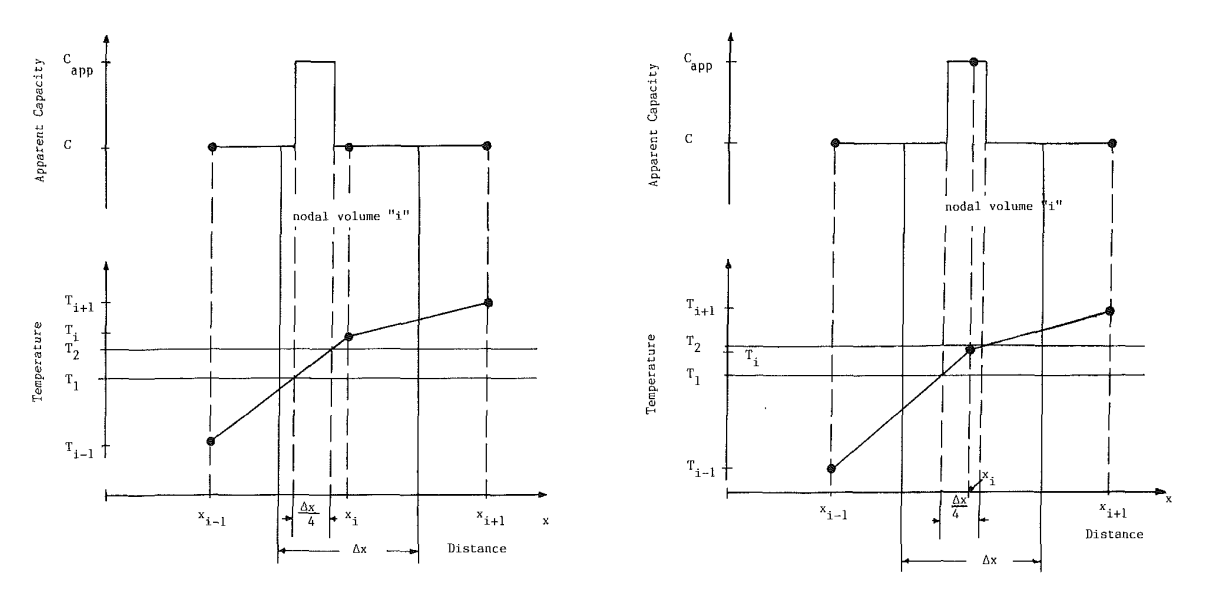
\includegraphics[width=.7\linewidth]{figures/chapter_3/EffectiveHeatCapacity.png}
    \caption{Heat capacity across a 1D element \cite{Poirier_Salcudean_1988}. Element failing to capture mushy-zone (left), and an element whose node captures the apparent heat capacity (right)}
    \label{fig:effective_heat_capacity_method}
\end{figure}
